% !TEX encoding = UTF-8 Unicode
\section{Auswertung}
In diesem Kapitel werden die im Kapitel \ref{loesungsskizze} vorgestellten Konfigurationen verwendet und eine Auswertung der VPN Verbindung von Firma B(Client) zur Firma A(Server) gemacht.\newline
Um die VPN Verbindung zu starten wird zuerst der Server mit Hilfe des Befehls ''openvpn /etc/openvpn/server.conf'' gestartet. Nach dem der Server gestartet wurde, wird bei Firma B der Client mit ''openvpn /etc/openvpn/client.conf'' gestartet. Dabei initiiert der Client den Verbindungsaufbau. 
\begin{figure}[h]
	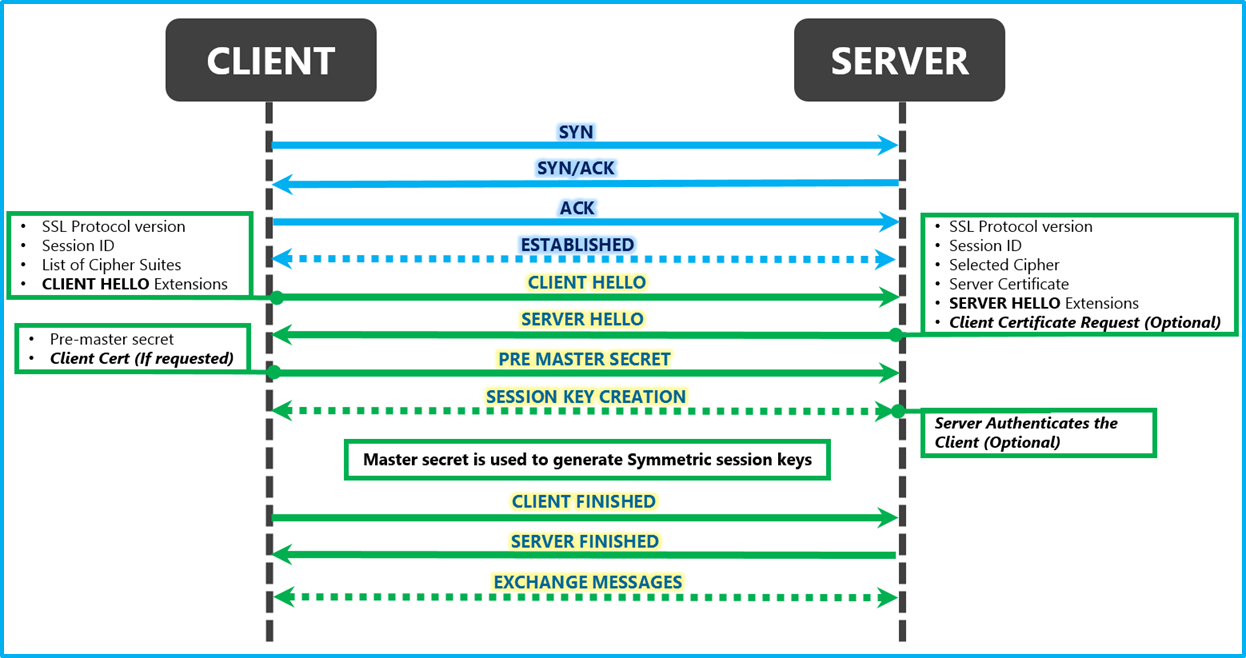
\includegraphics[width=\textwidth]{pictures/vpnVerbindungsaufbau.png}
	\caption{Verbindungsaufbau eines VPN's\cite{vanRijn2018May}}
	\label{fig:SSlhand}
\end{figure}
Die Abbildung \ref{fig:SSlhand} stellt drei Wege SSL Handshake zwischen Client und Server dar. Dabei wird zu Beginn eine unverschlüsselte Verbindung aufgebaut, indem dem Client die Server-IP und der Port mitgeteilt wird. Nachdem diese Verbindung ''ESTABLISHED'' ist, sendet der Client einen ''Client Hallo'' auf die nun bekannte IP-Adresse und den Port. Dabei liefert er das von ihm verwendete SSL Protokoll, eine Session ID, eine Liste von Chiffren, die er verwenden kann an den Server aus. Auf dieses ''Hallo'' sendet der Server selbst ein ''Server Hallo'' und liefert dabei dem Client ebenfalls seine SSL Protokoll Version, die Session ID, das von ihm gewählten Chiffre, sein Serverzertifikat und gegebenenfalls seine CCR (Client Certificate Request) aus. Hat der Client den ''Server Hallo'' erhalten, überprüft dieser die Gültigkeit, das Vertrauen in die CA und den öffentlichen Schlüssel mit der digitalen Signatur. 

Wenn er dies überprüft hat, erzeugt der Client, mit Hilfe des öffentlichen Schlüssels des Servers, ein Pre-master-secret. Dieses Secret sendet er nun an den Server. Der Server entschlüsselt das Pre-master-secret und anschließend erstellen Server und Client aus dem pre-master-secret einen symmetrischen Schlüssel, über den die Kommunikation verschlüsselt und entschlüsselt werden kann.\newline
Im Labor stießen wir auf ein nicht zu überbrückendes Hindernis. Dies entstand nach dem TCP-Handshake, im SSL-Handshake. Dabei konnte der Server sein ''Server Hallo'' nicht an den Client zurückschicken, was zur Folge hatte, dass der Client kein pre-master-secret erstellen konnte und der Vorgang abgebrochen wurde. Dieser Vorgang wurde nach 120 Sekunden erneut angestoßen und es wurde ein erneuter Verbindungsversuch unternommen, jedoch mit dem gleichen Resultat. Dieser Vorgang wird durch die Abbildung \ref{fig:logClient} und Abbildung \ref{fig:logServer} deutlich. 
\begin{figure}[h]
	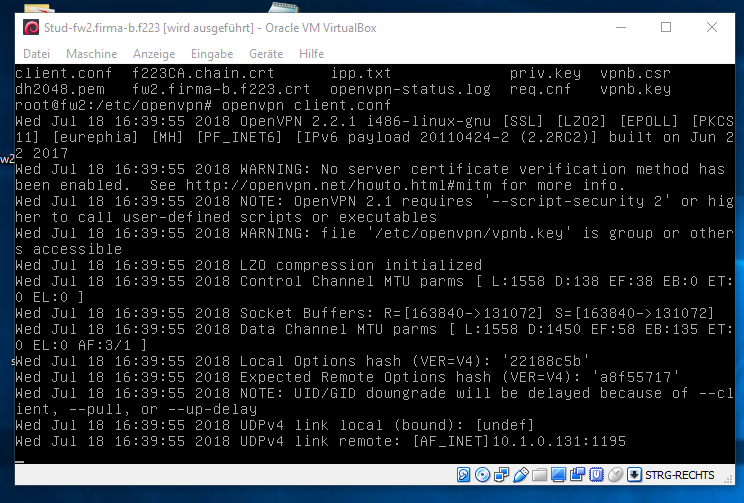
\includegraphics[width=\textwidth]{pictures/clientlog.png}
	\caption{Log Ausgabe des gestarteten VPN-Client}
	\label{fig:logClient}
\end{figure}
\begin{figure}[h]
	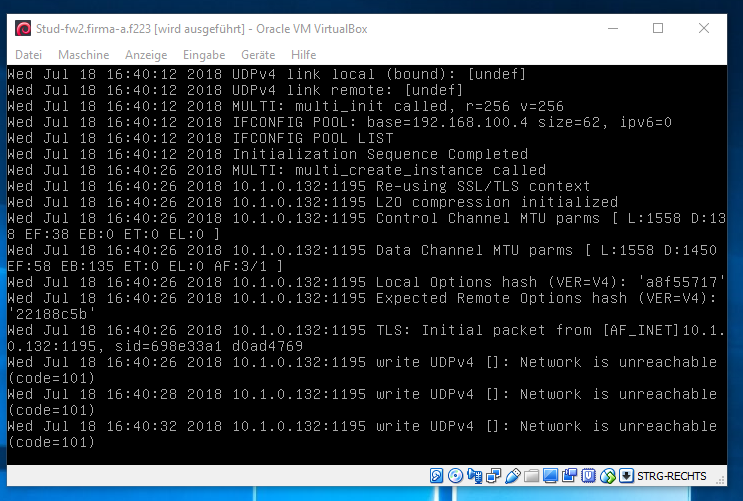
\includegraphics[width=\textwidth]{pictures/Serverlog.png}
	\caption{Log Ausgabe des gestarteten VPN-Servers}
	\label{fig:logServer}
\end{figure}
Nach Stunden der Fehlersuche und Neukonfiguration auf verschiedenen Systemen trat der Fehler erneut auf. Dies erhärtet die Vermutung, dass der Fehler in den Konfigurationen der virtuellen Maschinen zu finden sein könnte. Diese Vermutung konnte allerdings nicht bestätigt werden.  